\chapter[System Description]{System Description}
\label{chap:descricaoproblema}


\section{EHDA}
\label{sec:ehda_resume}

The electrospraying of liquids herein is referred to as electrohydrodynamic atomization (EHDA). The atomization by primarily electrical (electro) forces of a liquid (hydro) that is moving (dynamic) during the atomization captures the essence of the phenomena.\cite{Grace}
That motion applies to the liquid certain velocity that is not enough to create the spray alone. Therefore, the eletric field itself is the responsible for the spraying dynamics.\cite{prunet}

The stable balance between the capilary and field forces on the liquid suggest a \emph{quasi static} dynamics.
For this reason with a controlled enviroment we can reach a certain stable spraying mode as can be seen in the Figure \ref{fig:ehda_setup_ex2}.

\begin{figure}[H]
  \centering
  \resizebox{80mm}{!}{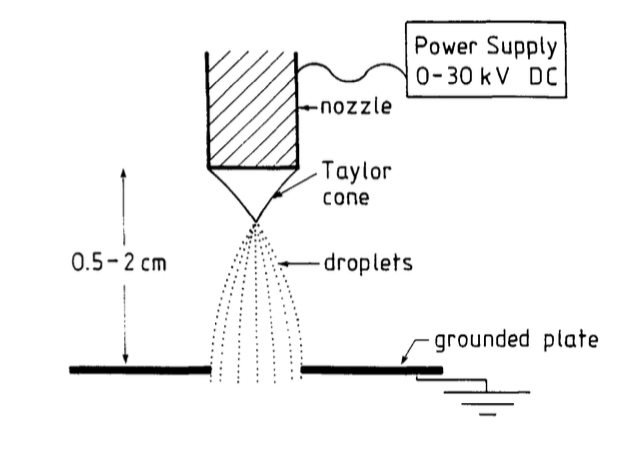
\includegraphics{Figuras/ehda_ex_2.png}}
  \caption{EHDA physical concept \cite{Gabriel}}
  \label{fig:ehda_setup_ex2}
\end{figure}

\section{Spraying modes}
\label{sec:spraying_modes_subsec}

Since 1915 with his pioneering work in EHDA, Zeleny observed several functioning modes with very different characteristics.
Years later the same phenomena was noticed by other scientists but the classification of these modes were still not well defined by the community.
For that Cloupeau and Prunet-Foch proposed spray mode classifications based in what they have seen experimentally and it's still being used as basis for EHDA researchs.\cite{prunet}

The Figures \ref{fig:dripping_camera_example}, \ref{fig:cone_camera_jet_example}, \ref{fig:multi_camera_jet_example} shows the 3 spraying dynamics that we are most intersted in this project. 

\begin{multicols}{3}

  \begin{figure}[H]
      \center
      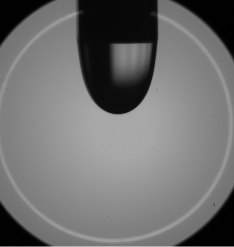
\includegraphics[width=3cm]{Figuras/drippingexample.png}
      \label{fig:dripping_camera_example}
      \caption{Dripping}
  \end{figure}


  \begin{figure}[H]
      \center
      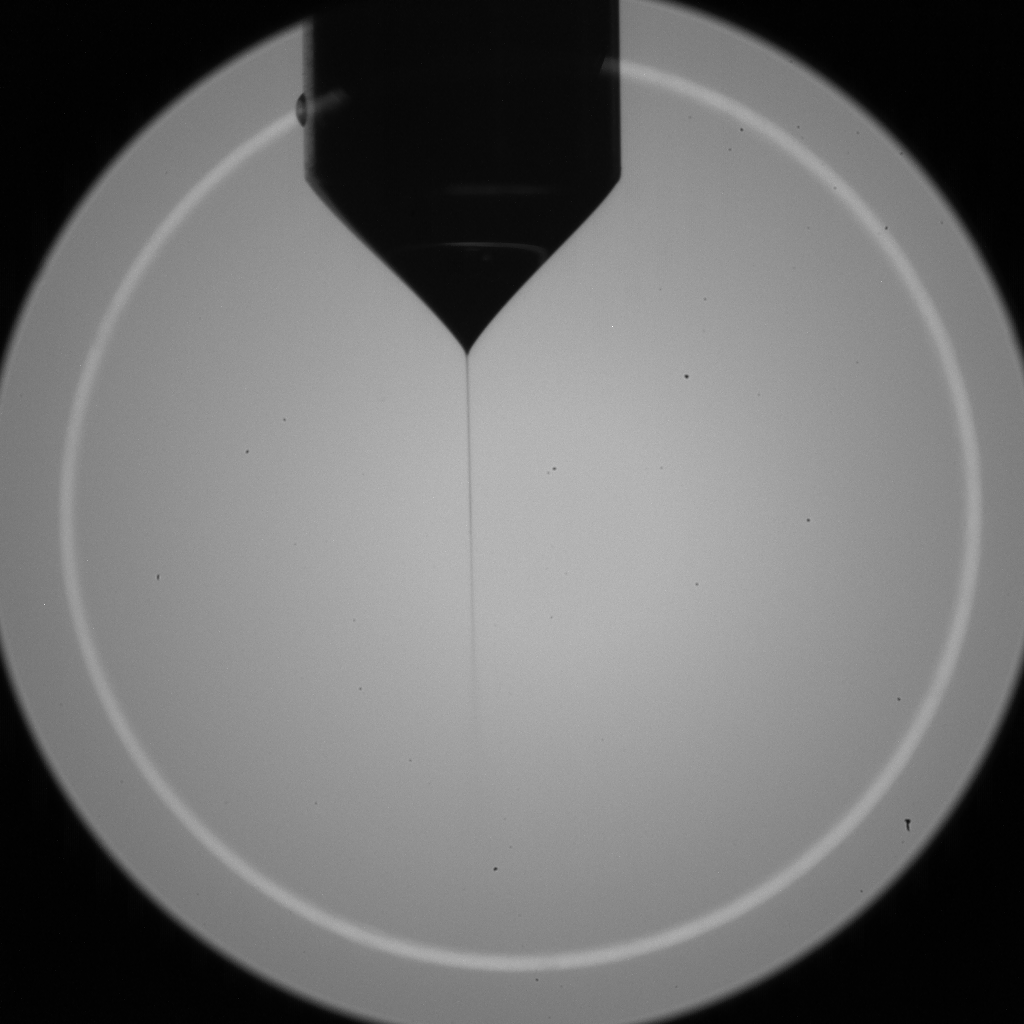
\includegraphics[width=3cm]{Figuras/conejetexample.png}
      \label{fig:cone_camera_jet_example}
      \caption{Cone Jet}
  \end{figure}


  \begin{figure}[H]
      \center
      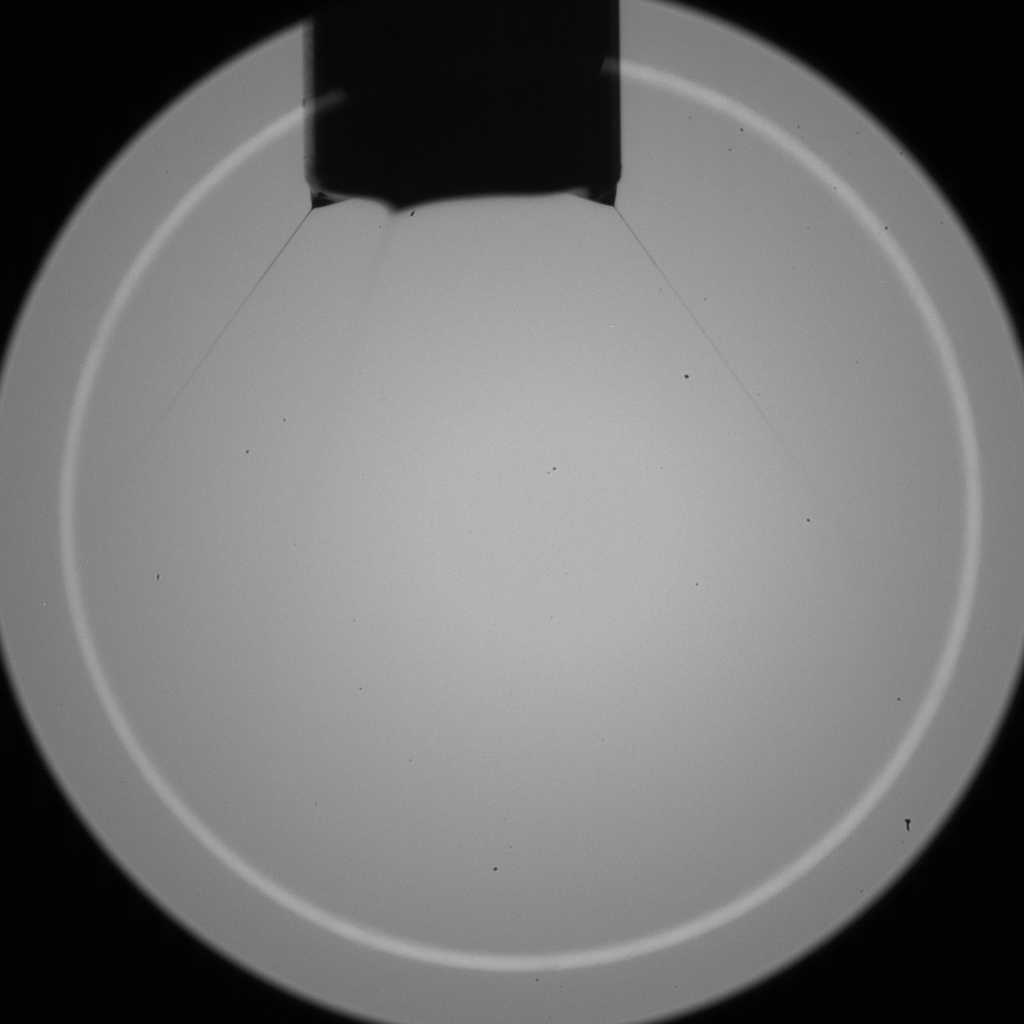
\includegraphics[width=3cm]{Figuras/multijetexample.png}
      \label{fig:multi_camera_jet_example}
      \caption{Multi Jet}
  \end{figure}

\end{multicols}

Through the various classifications defined we are going to work aggregating some of them and separating beetween 5 modes as shown above:

\subsection{Dripping}
\label{subsec:dripping}

In Dripping mode the eletric field applied is not enough to change the meniscus shape, phenomena called field enhanced dripping.
In that situation the liquid droplet has, in general, size bigger than the capilary and low frequency intervals between each drop.

\subsection{Intermittent}
\label{subsec:Intermittent}

Intermittent mode is defined when the eletric field forces starts to have a considerable effect in the meniscus and droplet formation. 
In this mode the droplet size is smaller than the nozzle, phenomena called microdripping, and the dripping frequency increases with the increasing of the field applied.

\subsection{Cone Jet}
\label{subsec:Cone Jet}

\subsection{Multi Jet}
\label{subsec:Multi Jet}

\subsection{Corona sparks}
\label{subsec:Corona sparks}







\section{Instrumentation}
\label{sec:instrumentation}

\subsection{Setup Organization}
\label{subsec:setup_organization}


\begin{figure}[H]
  \centering
  \resizebox{150mm}{!}{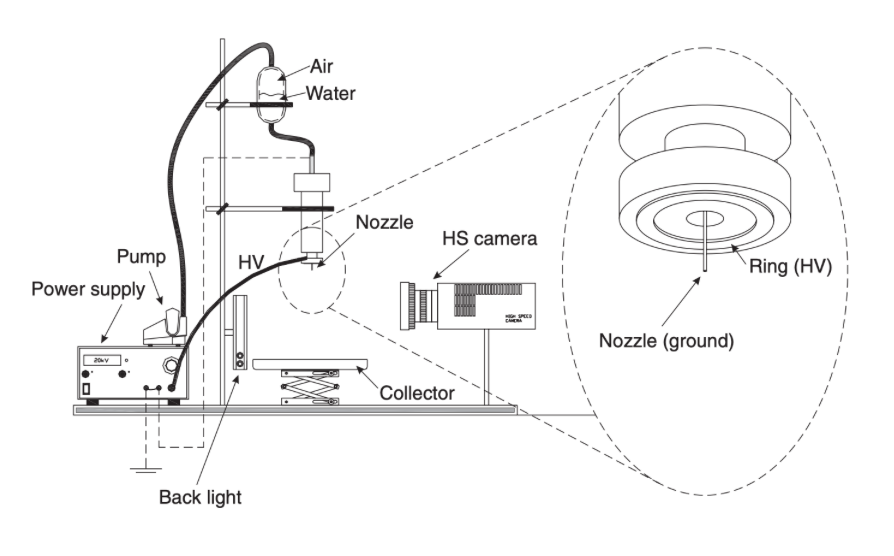
\includegraphics{Figuras/system_setup.png}}
  \caption{EHDA experiment setup \cite{Luewton}}
  \label{fig:ehda_setup}
\end{figure}


\begin{figure}[H]
  \centering
  \resizebox{150mm}{!}{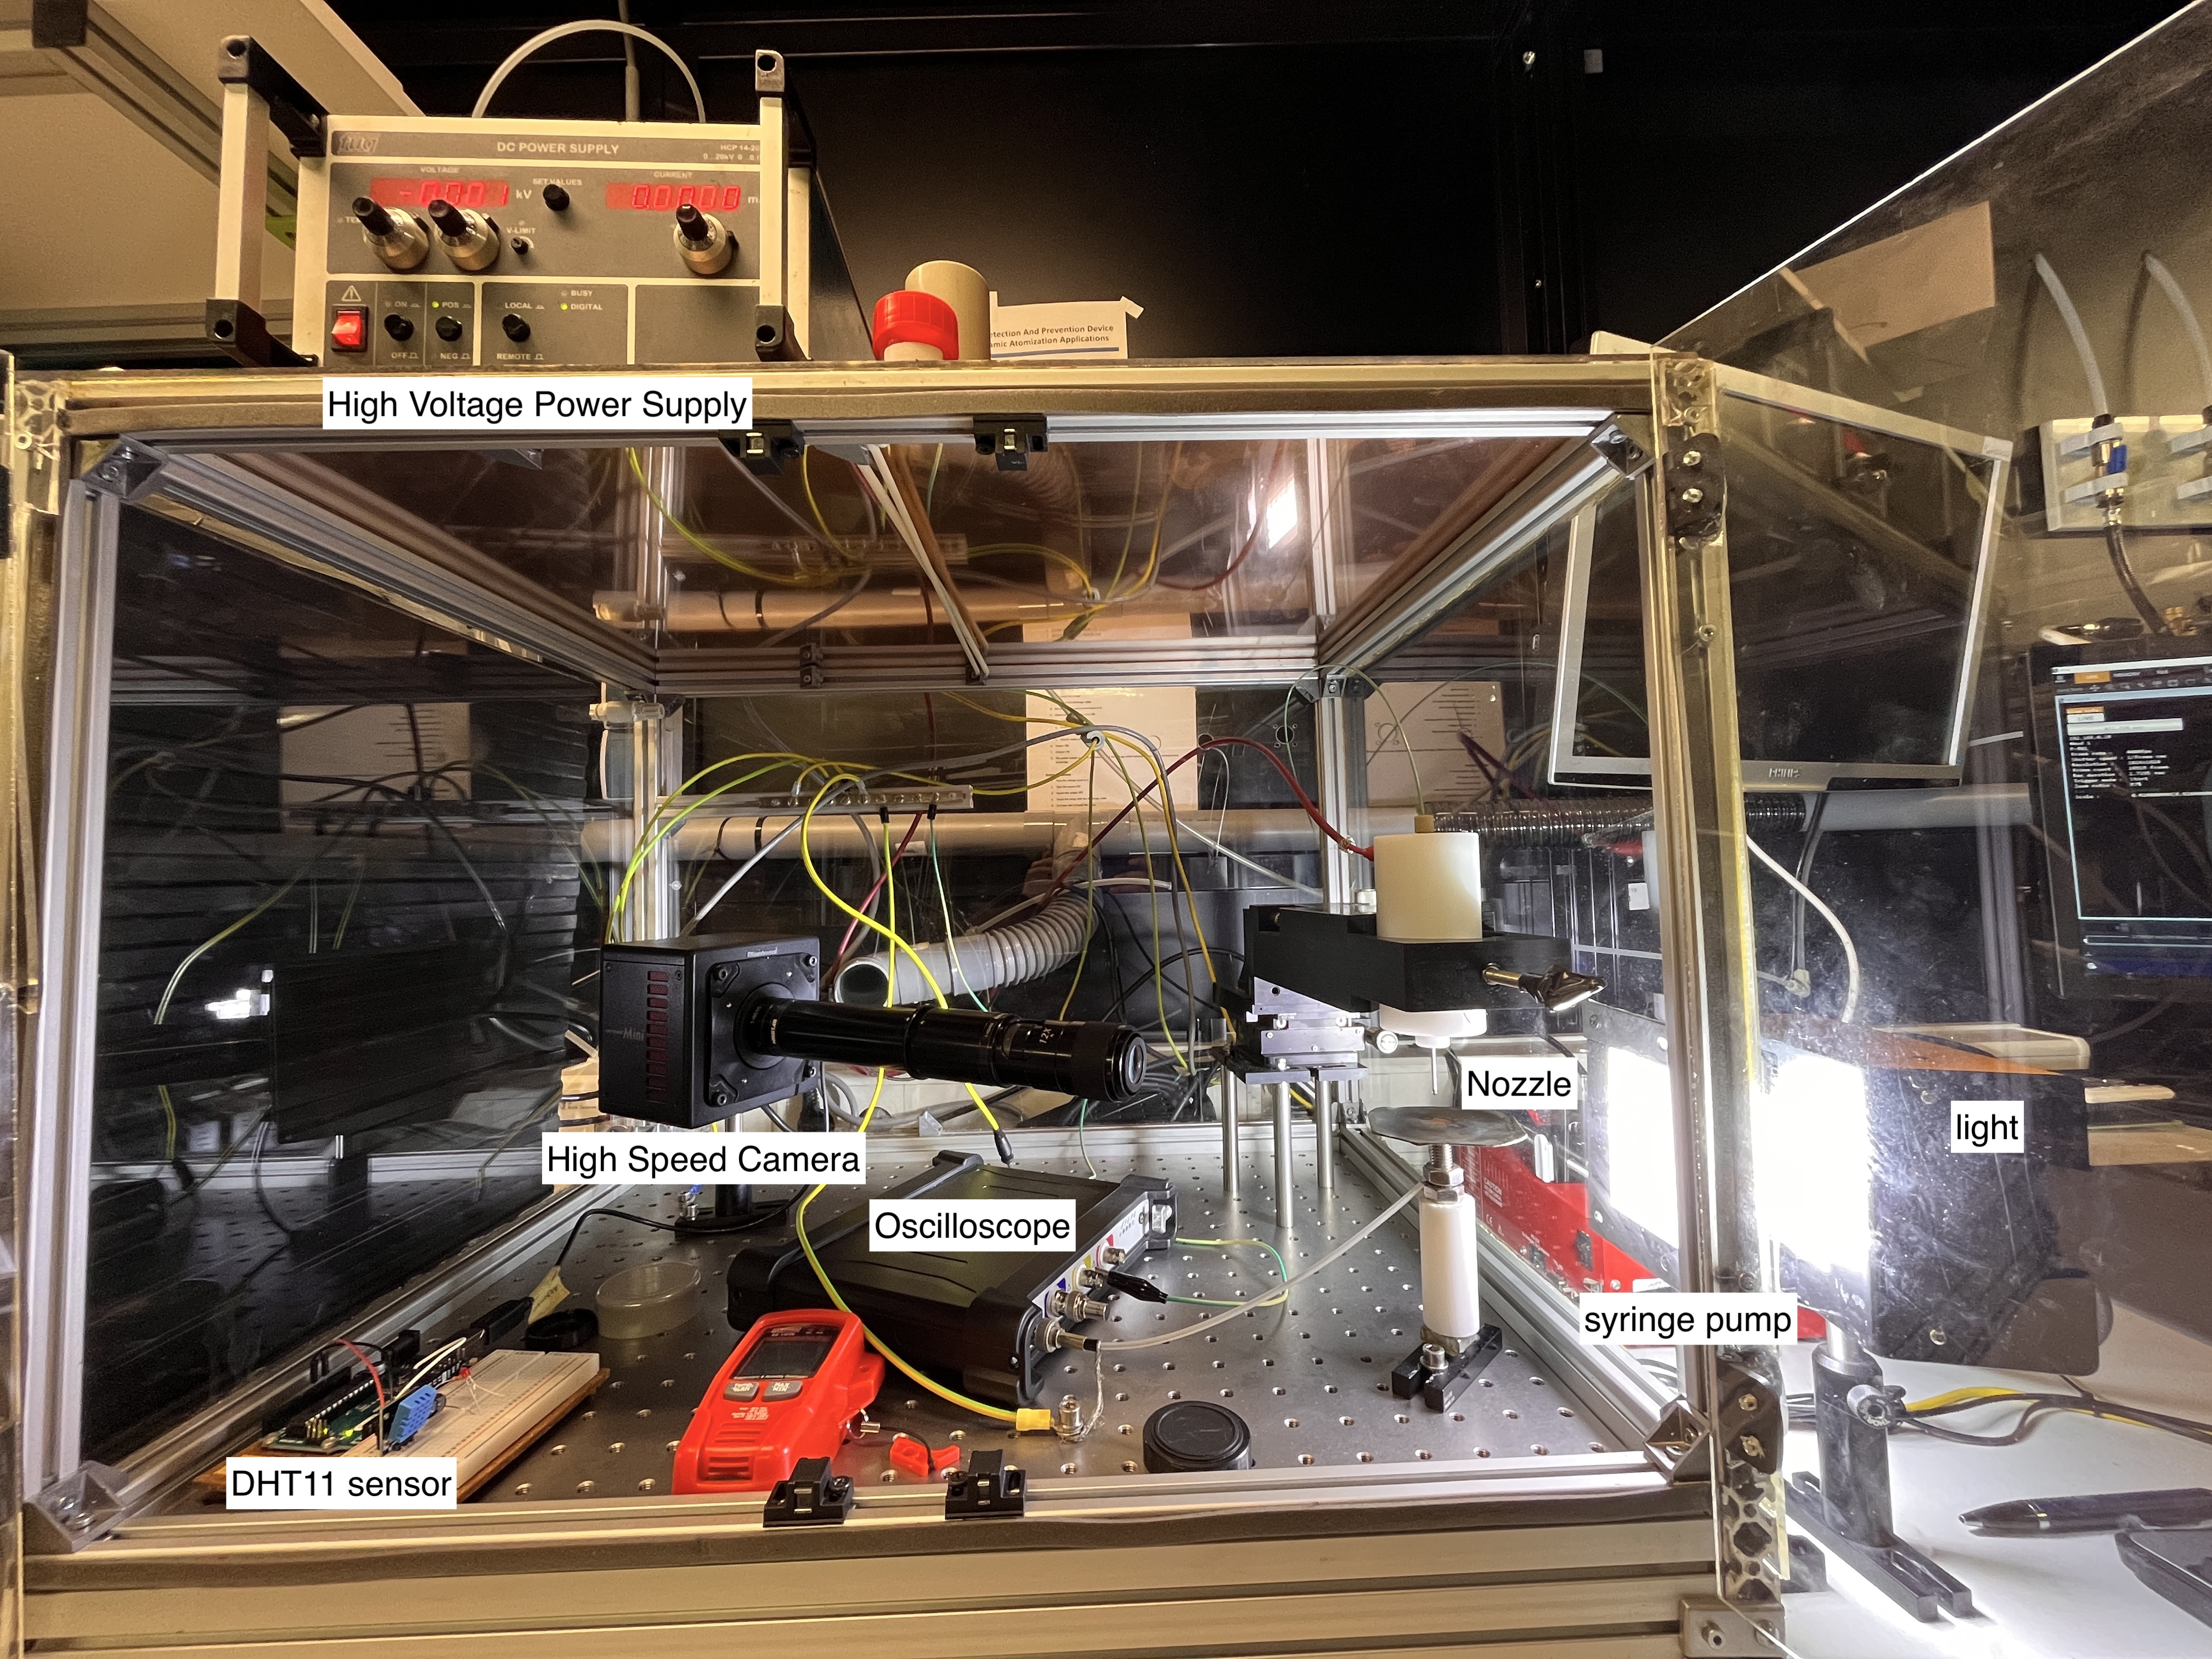
\includegraphics{Figuras/setup_pic.jpg}}
  \caption{EHDA automation system setup}
  \label{fig:setup_pic}
\end{figure}


\subsection{Instruments Used}
\label{subsec:instruments}

The peripherals automation routine was already developed by another student. In order to continue the research I took some time to understand the physical concept behind EHDA experiments and the project knowledge.
I made upgrades in the routine to include the high speed camera with a hardware triggering routine using an arduino microcontroler. This will be usefull to validate the further classification of the spray dynamics.


% ilustramos o processo com a Figura \ref{fig:setup}. 

\begin{figure}[H]
  \centering
  \resizebox{150mm}{!}{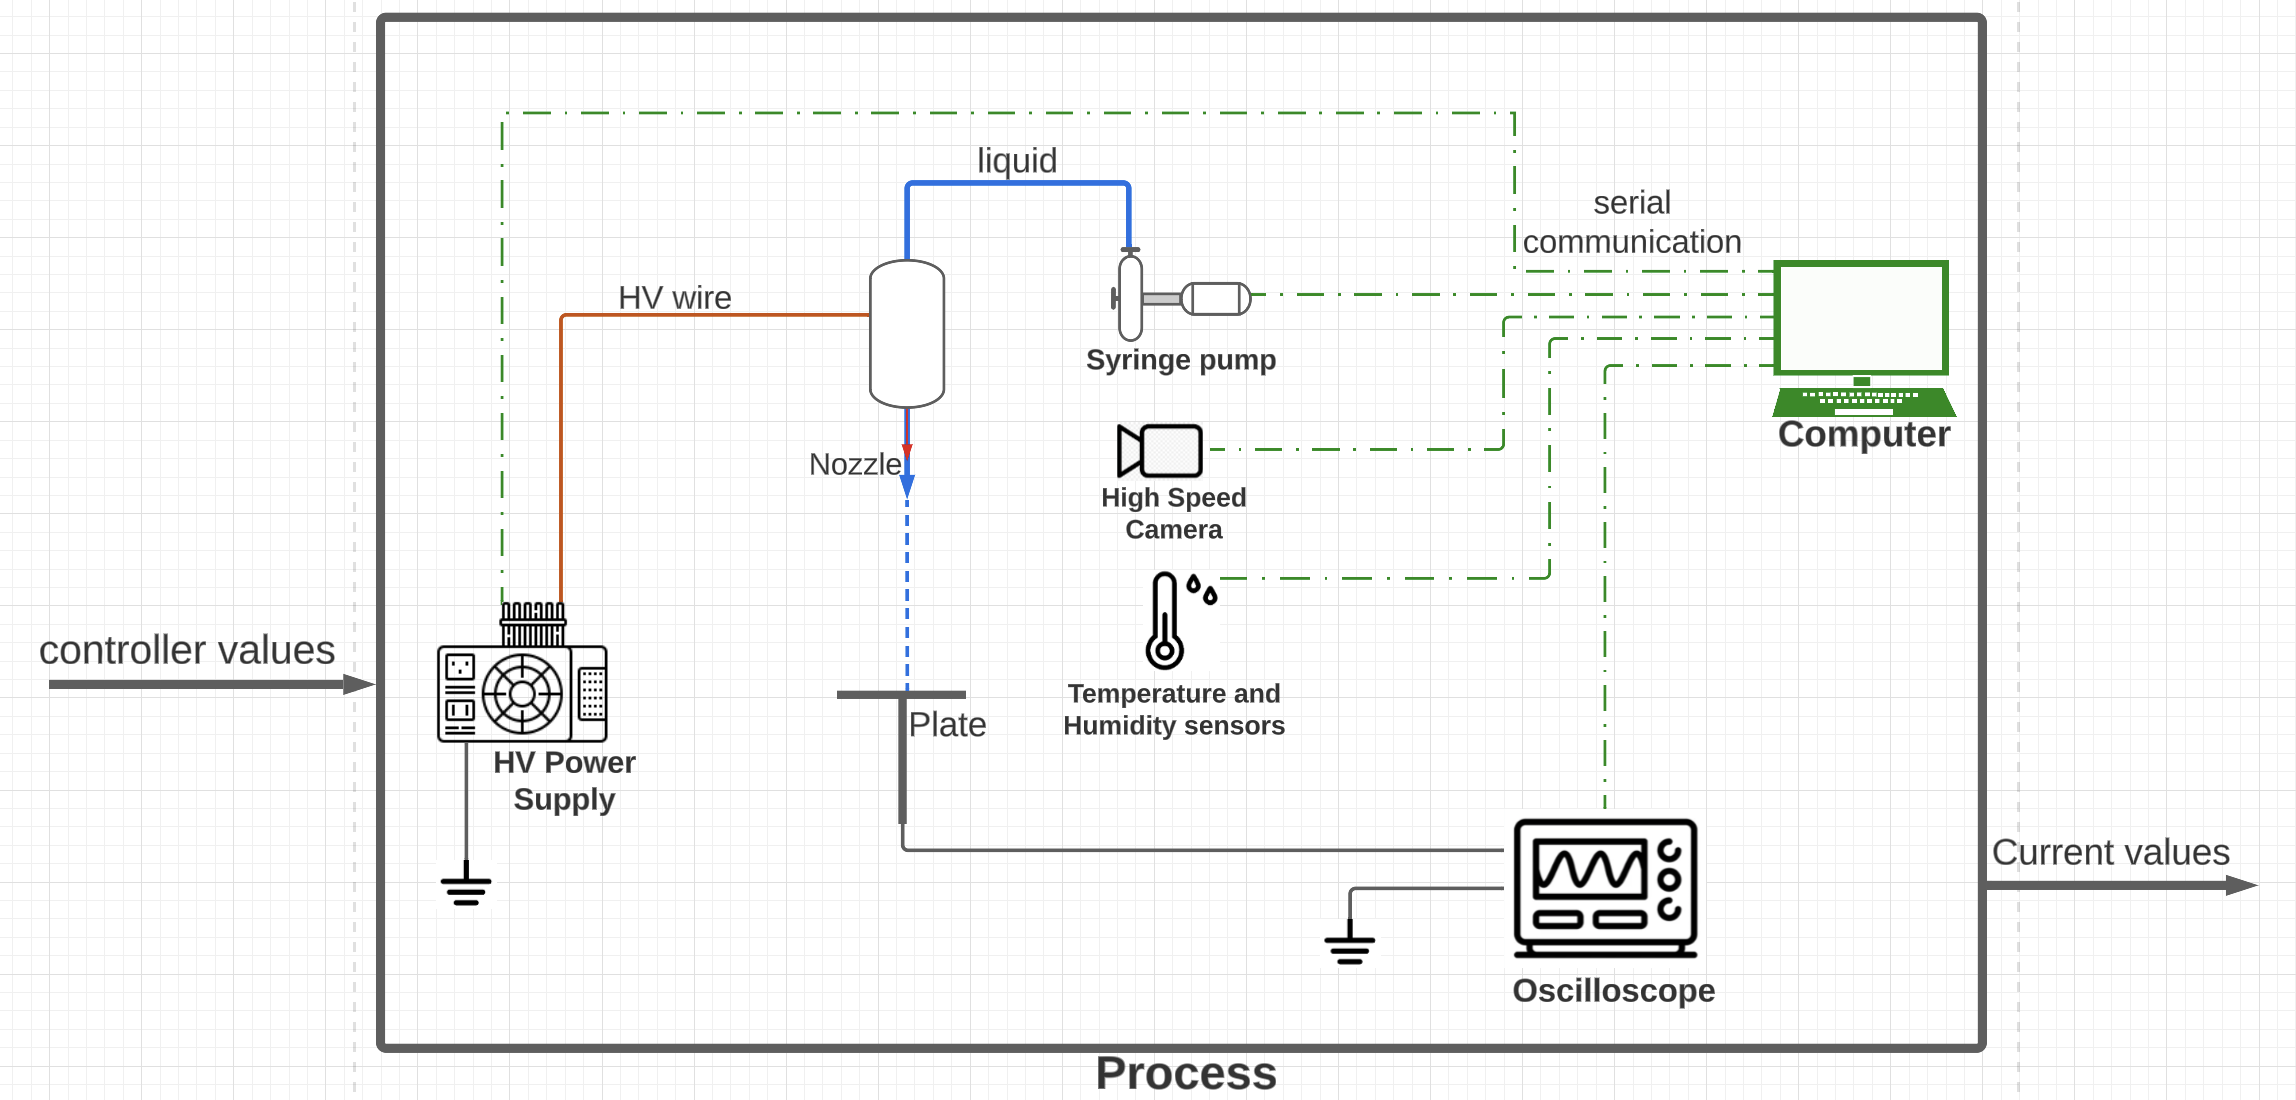
\includegraphics{Figuras/new_system_setup.png}}
  \caption{EHDA automation system setup}
  \label{fig:setup}
\end{figure}


\section{First Experiments}
\label{sec:first_experiments}

Initial tests were made to verify the setup assembly and the automation routine integration. In this step I could unterstand in practise how electrospray works.
I noticed that we need a large set of variables in the range to produce the desired dynamics of electrospray, which most of the time is cone-jet mode. Those variables can be the liquid properties such as surface tension, dielectric constant, viscosity, density, electrical conductivity and vacuum permitivity. And also physical variables such as flowrate, system impedance, system temperature, system humidity, nozzle to plate distance, nozzle dimensions and applied voltage.
The instruments used in the setup are:

\begin{enumerate}[a]
  \item High Voltage Power Supply (FUG)
  \item Oscilloscope TiePie WS6 DIFF 
  \item Humidity and Temperature sensor (DHT11 + Arduino Uno)
  \item High Speed Camera - Photron fastcam mini
  \item Syringe pump
  \end{enumerate}

\begin{figure}[H]
  \centering
  \resizebox{150mm}{!}{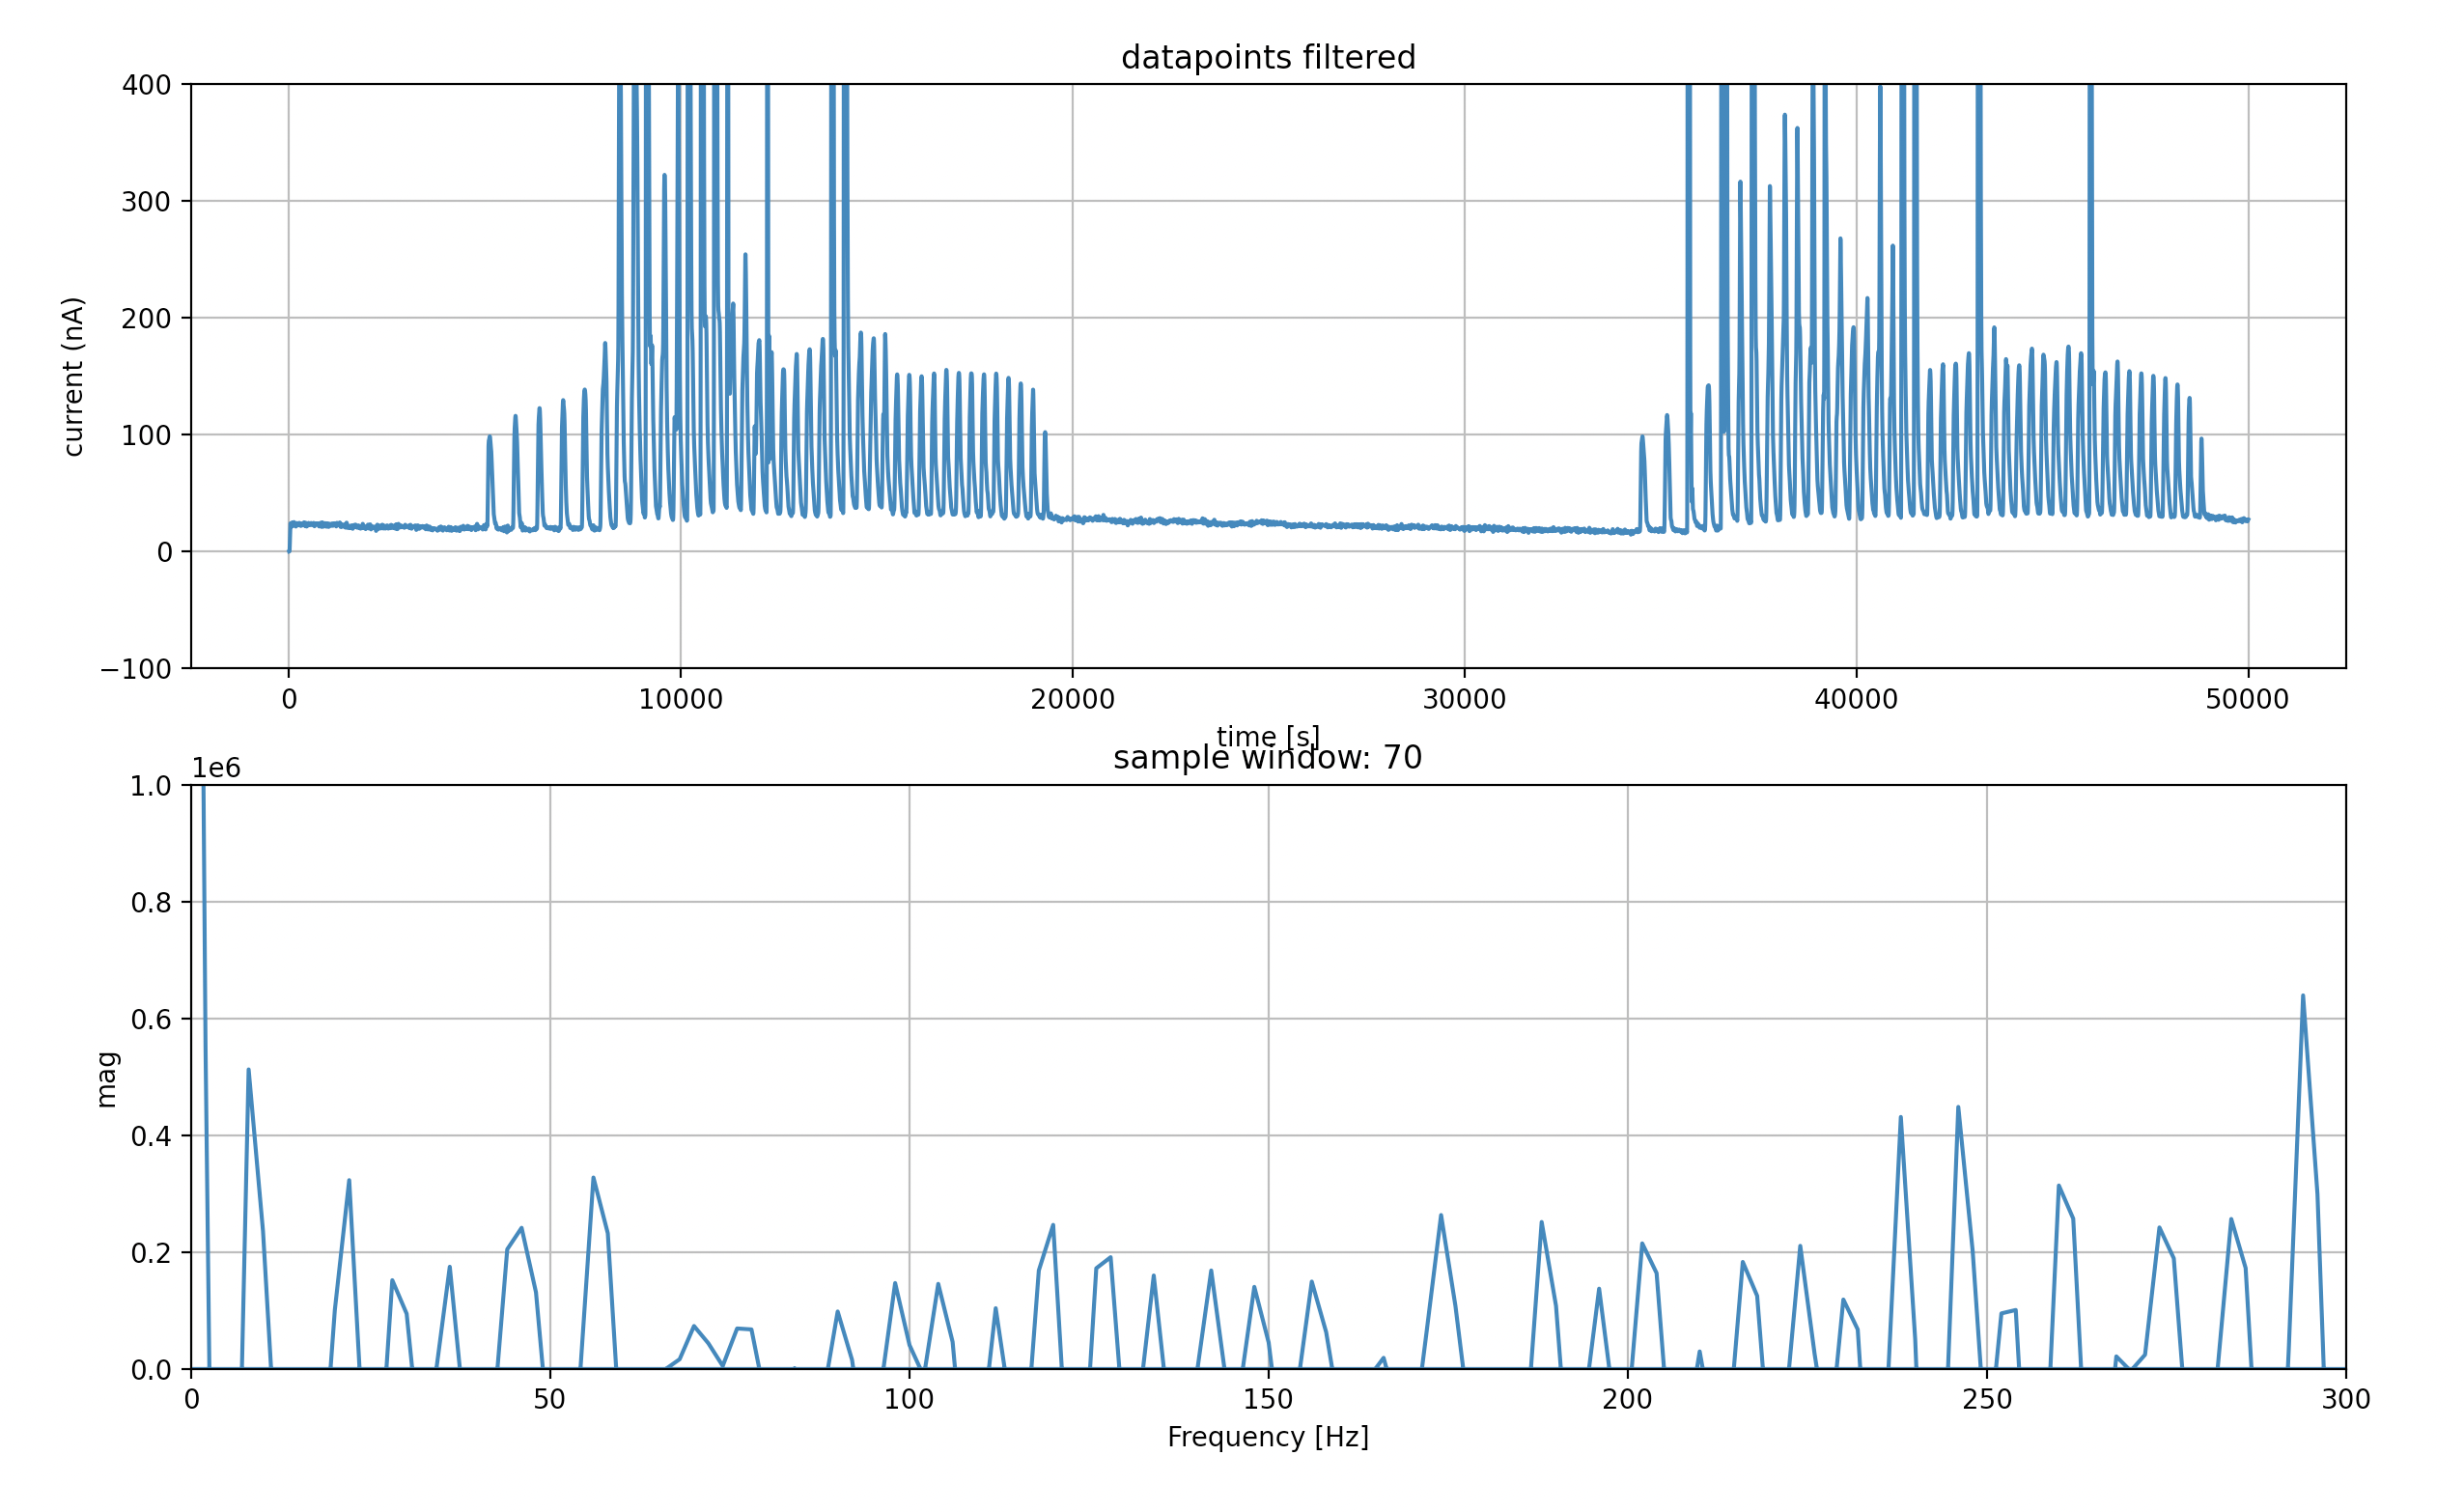
\includegraphics{Figuras/report2/img2.png}}
  \caption{EHDA automation system setup}
  \label{fig:microdripping_current_pic}
\end{figure}

\clearpage
